\documentclass[]{foi} 

\usepackage[utf8]{inputenc}
\usepackage{lipsum}

\vrstaRada{\projekt}

\title{Identificiranje korisnika pomoću dinamike tipkanja}
\predmet{\predmetSI}

\author{Karlo Vardijan, Lovro Pejaković, Filip Šoštarić, Stanko Smrček} 

\spolStudenta{\musko} 

\mentor{Bogdan Okreša Đurić}
\spolMentora{\musko} 
\titulaProfesora{dr. sc.}

\godina{2024}
\mjesec{ožujak}

\indeks{0016147086, 0016150223, 0016149647, 0016149535}

\smjer{Informacijsko i programsko inženjerstvo}


\sazetak{Dinamika tipkanja primjer je ponašajne biometrijske karakteristike koji se može koristitiu svrhu identifikacije i autentifikacije. Modernim algoritmima umjetne inteligencije, specifično strojnog i dubokog učenja, moguće je koristiti specifičnosti dinamike tipkanja korisnika u svrhu otkrivanja identiteta. Kroz praktični primjer demonstrirat će se način na koji identifikacija dinamikom tipkanja funkcionira te će se kroz analizu rezultata donjeti zaključak o korištenju spomenute biometrijske karakteristike u praksi.}
% abstract of 100 to 300 words.

\kljucneRijeci{dinamika tipkanja, biometrija, identifikacija, umjetna inteligencija, strojno učenje}
% keywords including 7 +/- 2 syntagms

\acrodef{VAS}{višeagentni sustav}



\begin{document}

\maketitle

\tableofcontents

\makeatletter \def\@dotsep{4.5} \makeatother
\pagestyle{plain}



\chapter{Uvod}

Cilj ovog projekta je analizom dinamike tipkanja identificirati korisnika. U ovom radu opisat će se sama dimanika tipkanja kao biometrijska karakteristika, u kojim područjima se primjenjuje i karakteristične mjere koje pohranjujemo te pomoću kojih na kraju vršimo samo identifikaciju. Biti će spomenuti sigurnosni rizici vezani za uporabu dinamike tipkanja i algoritmi strojnog učenja koji se koriste kod identifikacije. Detaljnije će se opisati metoda odabrana za praktični dio projekta. Na kraju slijedi opis implementiranog sustava za identifikaciju korisnika pomoću dinamike tipkanja. Analizirat će se rezultati dobiveni korištenjem implementiranog rješenja te odabranog seta podataka u svrhu identifikacije.

\chapter{Dinamika tipkanja kao biometrijska karakteristika}
Identifikacija je proces određivanja identiteta osobe bez prethodne deklaracije od strane osobe koju pokušavamo identificirati.\cite{Kasprowski2022} Identifikacija se može smatrati kao 1 naprema više veza jer iz nekog skupa korisnika pokušavamo odrediti kome pripadaju karakteristike pomoću kojih vršimo sam proces identifikacije. Značajke koje se koriste u biometriji se dijele na fizičke i ponašajne. Fizičke uključuju stvari poput otiska prsta i strukture lica dok ponašajne obuhvaćaju način hoda, glas, potpis te dinamiku tipkanja.\cite{Kasprowski2022}

Za razliku od fizičkih karakteristika koje su unikatne od osobe do osobe, ponašajne karakteristike se mijenjaju tijekom vremena te nisu toliko pouzdane što se tiče sigurnosti. Ponašajne karakteristike su obično implementirane kao potpora fizičkim. Na ponašajne karakteristike utječu stvari poput emocionalnog stanja osobe, zdravstvenih uvjeta te uvjeta okoline. Gore navedene stvari su primjenjive na dinamiku tipkanja koja je fokus ovog projekta. Obje vrste karakteristika moraju ispunjavati uvjete koje biometrijske karakteristike trebaju imati. To su jedinstvnenost, univerzalnost, lakoća prikupljanja, nepromjenjivost i prihvatljivost.\cite{Kasprowski2022} Jedinstvenost kaže da bi karakteristika trebala biti jedinstvena za osobu tj. dvije osobe nebi smjele imati identičnu mjeru neke značajke. Univerzalnost znači da bi sve osobe morale posjedovati tu značajku. Značajka bi trebala biti lako prikupljiva te se nebi trebala mijenjati kroz vrijeme. Također mora biti korisničko prihvatljiva. Sama dinamika tipkanja nije jedinstvena jer je moguće da dvije osobe tipkaju na isti način jer je to ponašajna karakteristika. Osim toga još neki problemi dinamike tipkanja su da se dinamika tipkanja može mijenjati ako smo bolesni, umorni ili ako koristimo dugačiju tipkovnicu nego inače \cite{Chang2021}. Osim ovih nedostataka dinamika tipkanja ima i dosta prednosti naprema nekim drugim biomatrijskim karakteristikama. Prednost je da netrebamo specijalne alate za prikupljanje dinamike tipkanja već korisnik tipka kao i inače, a pozadinski program skuplja podatke o tipkanju pa je zato dinamika tipkanja nenametljiva karakteristika \cite{Chang2021}. Dobar potencijal za dinamiku tipkanja je kod autetifikacije sa lozinkom u kojem dinamika tipkanja može biti drugi faktor koji se provjerava kako bi se bolje zaštitio račun korisnika jer čak ako napadač zna lozinku korisnika dinamiku tipkanja je teško lažirati. Isto tako potencijal za dinamiku tipkanja je da se nakon autentifikacije kontinuirano provjerava dinamika tipkanja korisnika i ako je drukčija nego inače može se otkritit napadač koji je uspio upasti u sustav korisnika.

Prvi primjeri korištenja dinamike tipkanja u svrhu identifikacije pojavili su se tijekom 2. Svjetskog Rata kod slanja poruka Morsovim kodom. Način na koji je poruka otipkana mogla je dati uvid u legitimnost poruke \cite{Haring2007}. U tom smislu dunamika tipkanja je relativno nova biometrijska karakteristika koja još nije puno istražena i ne postoje puno sustava koji ih koriste. 

Postojeća rješenja i implementacije bazirane su na statističkim podacima određenih događaja. Događaji koji se uglavnom koriste su duljine trajanja između pritiska i odpuštanja jedne tipke (eng. Dwell time), vrijeme koje protekne između odpuštanja jedne te pritiska druge tipke (eng. Interval), vrijeme između otpuštanja prve te odpuštanja druge tipke (eng. Up to up), vrijeme između pritiska prve tipke te pritiska druge (eng. Flight time), vrijeme između pritiska prve tipke te odpuštanja druge scenariji u kojima se koriste "Shift" i "Capslock" tipke za pisanje velikih slova i korištenje strelica za pozicioniranje u tekstu.\cite{Kasprowski2022} Manje korištene značajke uključuju i poziciju prsta na tipkama što zahtjeva korištenje kamere. Također se može promatrati i odabir prstiju koji se koristi za određene tipke za koje je također potrebna kamera. Druga klasifikacija obuhvaća metrike kao što su Down-down time, Up-down time, Up-up time te Down-up time koje jednostavno opisuju vremenski razmak između otpuštanja (Up) ili pritiska (Down) prve tipke te otpuštanja ili pritiska druge.

Kod procesa identifikacije koriste se dvije vrste tekstova: oni s definiranim brojem znakova i oni s nasumično odabranom duljinom. Prva opcija je primjenjuje u većini istraživanja koja su povezana s dinamikom tipkanja. Fokus je stavljen na odabir odgovarajućih algoritma te njihovo poboljšanje. Drugi pristup se koristi za kontinuiranu autentifikaciju.\cite{Kasprowski2022} Podaci o dinamici tipkanja se obično prikupljaju tipkovnicom, no kako su pametni mobiteli u današnje vrijeme sveprisutni, moguće je i na taj način obaviti prikupljanje. Ovdje također možemo zabilježiti točne koordinate pritiska, veličinu ekrana koju prst prekriva kod određene tipke te jačinu pritiska.\cite{Lee2018}

\begin{figure}[!h]
    \centering
    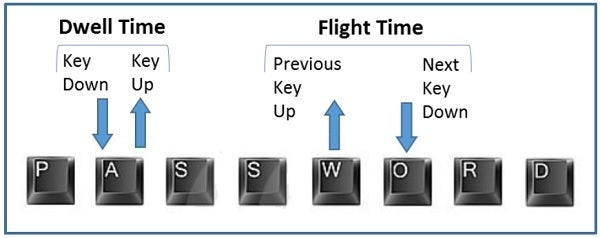
\includegraphics[width=0.6\textwidth]{slike/karakteristike.jpeg}
    \caption{Slika prikaza karakterističnih vremena dinamike tipkanja; preuzeto iz \cite{Rootstrap}}
    \label{fig:slika-kar-vremena}
\end{figure}

\chapter{Skup podataka dinamičkog tipkanja}
Za ovaj rad pronašli smo besplatni skup podataka za dinamičko tipkanje KeyRecs. Skup podataka je dobiven od 99 sudionika koji su sudjelovali u dva zadatka  \cite{Dias2023}. Prvi zadatak je bio pisanje lozinke „vpwjkeurkb“ 200 puta kroz dvije sesija, a drugi zadatak je bio prepisivanje 10 odlomaka raznih literatura isto kroz dvije sesije \cite{Dias2023}. Ti zadaci su se provodili preko web stranice koja je bilježila razna vremena tijekom tipkanja \cite{Dias2023}. Vremena koja su se bilježila su: od pritiska tipke do puštanja tipke (DU), od pritiska tipke do pritiska druge tipke (DD), od puštanja tipke do pritiska druge tipke (UD), od puštanja tipke do puštanja druge tipke(UU), od pritiska tipke do puštanja druge tipke (DU) i ukupno vrijeme tipkanja \cite{Dias2023}. Ta vremena su dobro prikazana na slici \ref{fig:graf-vremena-tipkanja}. Osim tih vremena za svakoga korisnika su  zabilježene: godine, spol, nacionalnost i dominantna ruka  \cite{Dias2023}. Podaci za prvi zadatak pisanja lozinke su zapisani kao tablica \ref{tab:KeyRecs-podaci}. U svakom redu je zabilježeno: tko je pisao, koja je sesija, koje ponavljanje i vremena za svaku tipku sifre \cite{Dias2023}. Vremena su zabilježena u kolone (D|U).tipka1.tipka2 gdje prvi dio prikazuje određeno vrijeme na temelju slike \ref{fig:graf-vremena-tipkanja} a druga dva dijela na koju tipku se odnosi \cite{Dias2023}.

\begin{table}[!h]
    \centering
    \caption{Dio podataka iz KeyRecs skupa podataka; prema \cite{Dias2023}}
    \begin{tabularx}{1\textwidth}{|l|l|l|l|l|l|l|l|l|l|}
    \hline
        \cellcolor{gray!25}participant & \cellcolor{gray!25}session & \cellcolor{gray!25}repetition & \cellcolor{gray!25}DU.v.v & \cellcolor{gray!25}DD.v.p & \cellcolor{gray!25}DU.v.p & \cellcolor{gray!25}UD.v.p & \cellcolor{gray!25}UU.v.p & \cellcolor{gray!25}DU.p.p & \cellcolor{gray!25}... \\ \hline
        p001 & 1 & 1 & 0.129 & 1.917 & 1.804 & 2.046 & 1.933 & 0.113 & ... \\ \hline
        p001 & 1 & 2 & 0.112 & 0.192 & 0.096 & 0.304 & 0.208 & 0.096 & ... \\ \hline
        p001 & 1 & 3 & 0.088 & 0.253 & 0.182 & 0.341 & 0.27 & 0.071 & ... \\ \hline
        ... & ... & ... & ... & ... & ... & ... & ... & ... & ... \\ \hline
    \end{tabularx}
    \\[10pt]
    \label{tab:KeyRecs-podaci}
\end{table}


\begin{figure}[!h]
    \centering
    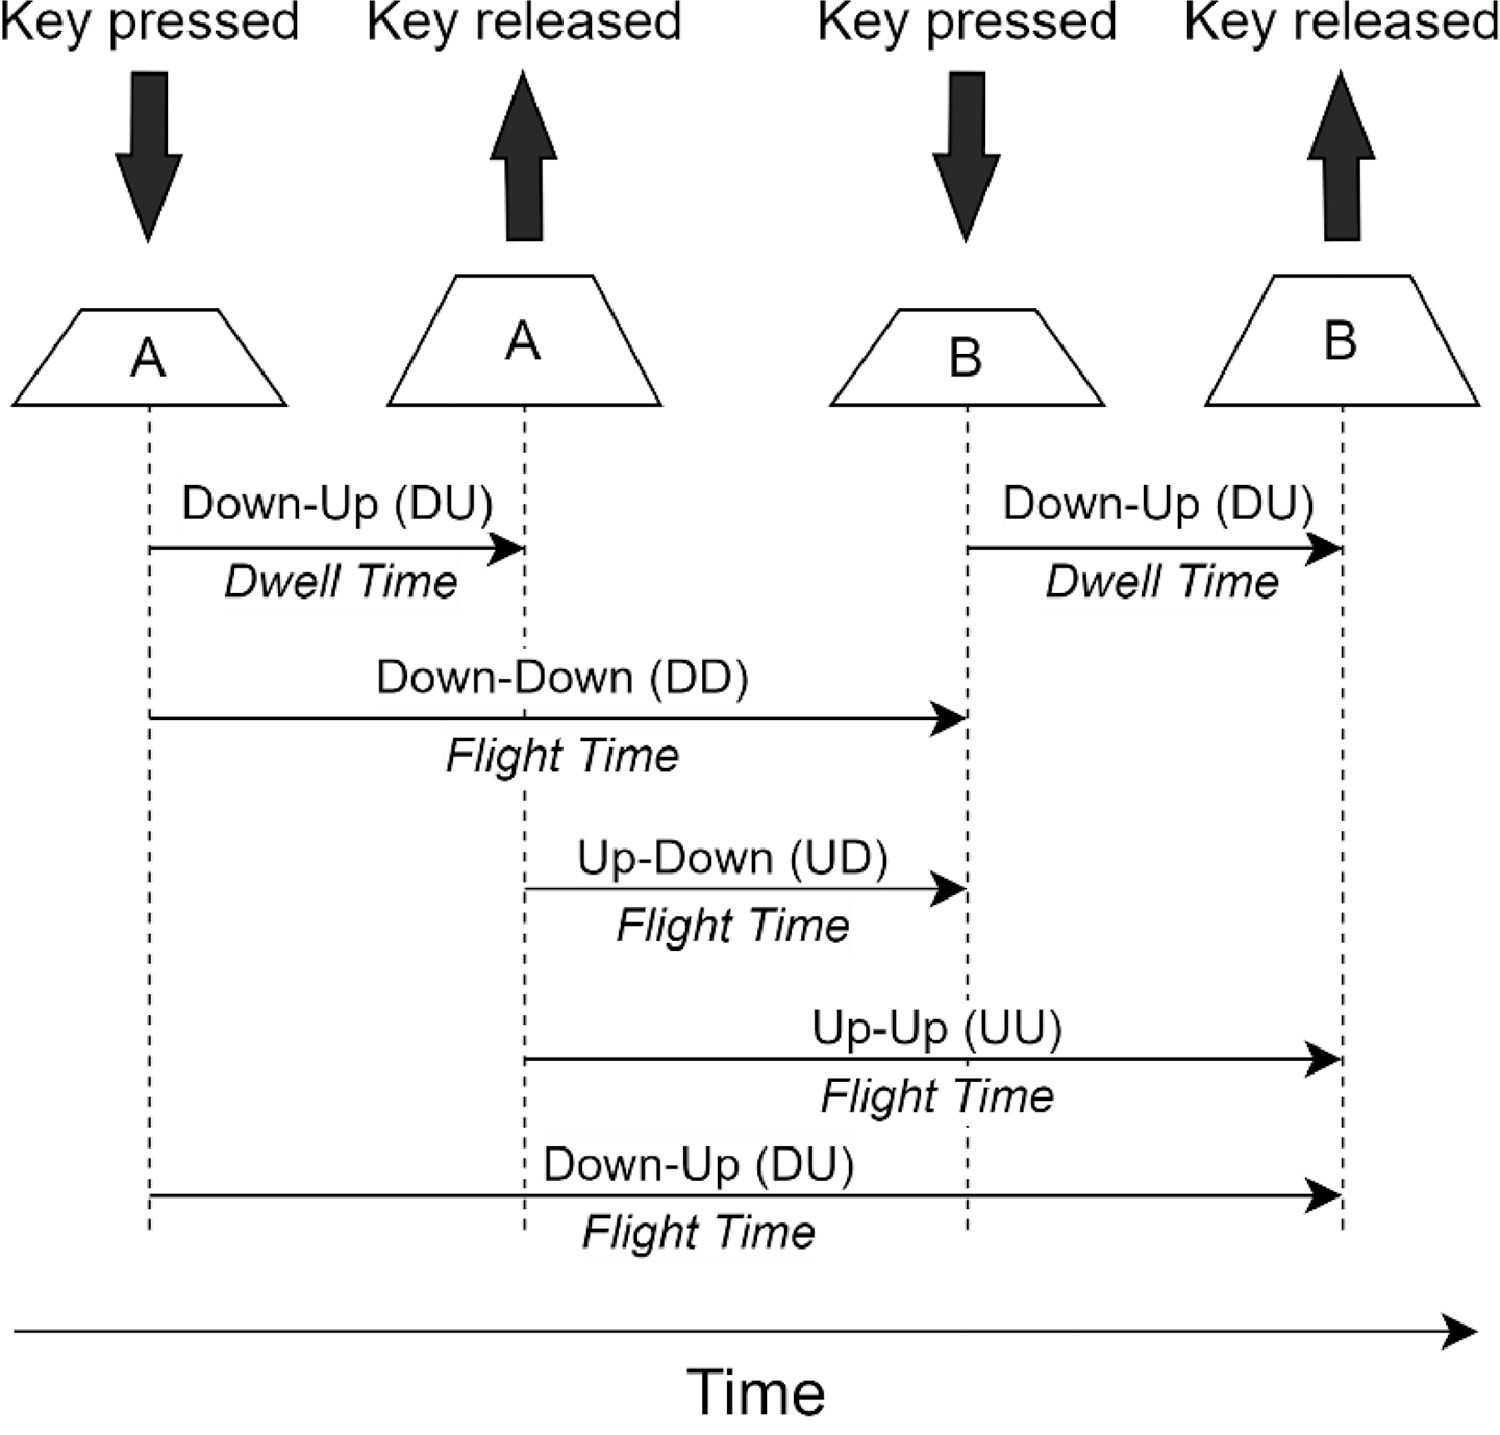
\includegraphics[width=0.6\textwidth]{slike/tipkanje-graf.jpg}
    \caption{Grafikon bilježenih vremena tijekom tipkanja; preuzeto iz \cite{Dias2023}}
    \label{fig:graf-vremena-tipkanja}
\end{figure}


\chapter{Metode analize dinamike tipkanja pomoću umjetne inteligencije}
Umjetna inteligencija i strojno učenje prikladan su način za obradu velike količine podataka koje je potrebno obuhvatiti kako bi sa dosta velikom sigurnošću mogli autenticirati korisnika. Metode se mogu svrstati u dvije kategorije, metode klasičnog strojnog učenja i metode dubokog učenja.

\section{Metode klasičnog strojnog učenja}
Strojno učenje (engl. Machine learning) je grana umjetne inteligencije (engl. Artificial intelligence) čiji je fokus na korištenju podataka i algoritama na način da imitiraju kako ljudi uče, postepeno poboljšavajući svoje rezultate \cite{ibmcom}. 
Algoritmi strojnog učenja organizirani su u sljedeće grupe: nadzirano učenje (engl. supervised learning), nenadzirano učenje (engl. unsupervised learning), polunadzirano učenje (engl. semi-supervised learning), učenje s pojačanjem (engl. reinforcement learning). 
Nadzirano učenje je vrsta strojnog učenja dobila gdje je stroj "nadgledan" dok uči, što znači da se algoritmu daju informacije kako bi mu se pomoglo u učenju. Definiran je korištenjem označenih podataka (engl. Labeled Data). Označeni podaci skup su podataka koji sadrži puno primjera značajki (engl. Features) i mete (engl. Target). Nadzirano učenje koristi algoritme koji uče odnos značajki i mete iz skupa podataka. Taj se proces naziva obukom ili treniranjem. \cite{Coursera2023}
Algoritmi za učenje bez nadzora ne koriste iste označene skupove za obuku i podatke. Umjesto toga, stroj traži manje očite uzorke u podacima. Strojno učenje bez nadzora korisno je kada treba identificirati obrasce i koristiti podatke za donošenje odluka. \cite{Coursera2023}
Polunadzirano učenje je relativno nova i manje popularna vrsta strojnog učenja koja, tijekom obuke, spaja znatnu količinu neoznačenih podataka s malom količinom označenih podataka. Polunadzirano učenje je između nadziranog učenja (s označenim podacima o osposobljavanju) i nenadziranog učenja (neoznačeni podaci o osposobljavanju). \cite{Datacamp}
Učenje s pojačanjem najbliža je vrsta strojnog učenja načinu na koji ljudi uče. Algoritam ili agent koji se koristi uči u interakciji sa svojom okolinom i dobivanjem pozitivne ili negativne nagrade. \cite{Coursera2023}

\subsection{K-Nearest Neighbours}
K-NN je neparametarski klasifikator s nadziranim učenjem. Moguće ga je koristiti za regresijski ili klasifikacijske probleme ali se tipično koristi kao klasifikacijski algoritam. Unutar klasifikacijskih problema on radi tako da se većinskim glasanjem odabire klasa koja je "najbliža" podacima danim za klasifikaciju. 

\subsection{Support Vector Machines}
Support Vector Machines (SVM) je nadzirani algoritam učenja koji se obično koristi za zadatke klasifikacije i prediktivnog modeliranja. SVM algoritmi su popularni jer su pouzdani i mogu dobro raditi čak i s malom količinom podataka. SVM algoritmi rade stvaranjem granice odluke koja se naziva "hiperravnina". U dvodimenzionalnom prostoru, ova hiperravnina je poput linije koja razdvaja dva skupa označenih podataka. 
Cilj SVM-a je pronaći najbolju moguću granicu odluke maksimiziranjem margine između dva skupa označenih podataka. Traži najširi jaz ili prostor između razreda. Svaka nova podatkovna točka koja padne s bilo koje strane ove granice odluke klasificirana je na temelju oznaka u skupu podataka za obuku. \cite{Coursera2024}

\subsection{Random Forest}
Random Forest algoritam je skup stabala odlučivanja koji se koriste za klasifikaciju i prediktivno modeliranje. Umjesto da se oslanja na jedno stablo odlučivanja, nasumična šuma kombinira predviđanja iz više stabala odluka kako bi napravila točnija predviđanja. U slučajnoj šumi, brojni algoritmi stabla odlučivanja (ponekad stotine ili čak tisuće) pojedinačno se treniraju pomoću različitih slučajnih uzoraka iz skupa podataka za obuku. Ova metoda uzorkovanja naziva se "slaganje u vrećice". Svako stablo odlučivanja trenira se neovisno na svom odgovarajućem slučajnom uzorku. 
Jednom obučena, nasumična šuma uzima iste podatke i unosi ih u svako stablo odlučivanja. Svako stablo daje predviđanje, a nasumična šuma zbraja rezultate. Najčešće predviđanje među svim stablima odlučivanja zatim se odabire kao konačno predviđanje za skup podataka. \cite{Coursera2024}

\section{Metode dubokog učenja}
Sposobnost računala da obavljaju neke složene zadatke - prikupljanje podataka sa slike ili videa, na primjer - još uvijek je daleko ispod onoga za što su ljudi sposobni. Modeli dubokog učenja uvode iznimno sofisticiran pristup strojnom učenju i spremni su za rješavanje ovih izazova jer su posebno modelirani prema ljudskom mozgu. Aplikacije dubokog učenja koriste slojevitu strukturu algoritama koja se naziva umjetna neuronska mreža (ANN). Dizajn takvog ANN-a inspiriran je biološkom neuronskom mrežom ljudskog mozga, što dovodi do procesa učenja koji je mnogo sposobniji od standardnih modela strojnog učenja. \cite{Wolfewicz}

\subsection{Convolutional Neural Networks}
Konvolucijska neuronska mreža (CNN) vrsta je algoritma dubokog učenja koji je posebno prikladan za zadatke prepoznavanja i obrade slika. Sastoji se od više slojeva, uključujući konvolucijske slojeve, slojeve za udruživanje i potpuno povezane slojeve. 
Konvolucijski slojevi ključna su komponenta CNN-a, gdje se filtri primjenjuju na ulaznu sliku kako bi se izdvojile značajke kao što su rubovi, teksture i oblici. Izlaz konvolucijskih slojeva zatim prolazi kroz skupne slojeve, koji se koriste za smanjivanje uzorkovanja mapa značajki, smanjujući prostorne dimenzije uz zadržavanje najvažnijih informacija. Izlaz slojeva udruživanja zatim prolazi kroz jedan ili više potpuno povezanih slojeva, koji se koriste za predviđanje ili klasificiranje slike. 
CNN-ovi se obučavaju pomoću velikog skupa podataka označenih slika, gdje mreža uči prepoznati obrasce i značajke koje su povezane s određenim objektima ili klasama. Jednom obučen, CNN se može koristiti za klasificiranje novih slika ili izdvajanje značajki za korištenje u drugim aplikacijama kao što je detekcija objekata ili segmentacija slike. \cite{GeeksforGeeks2020}

\subsection{Recurrent Neural Networks}
Rekurentna neuronska mreža (RNN) vrsta je umjetne neuronske mreže koja koristi sekvencijalne podatke ili podatke vremenskih serija. Zbog svoje unutarnje memorije, RNN-ovi mogu zapamtiti važne stvari o ulazu koji su primili, što im omogućuje da budu vrlo precizni u predviđanju onoga što slijedi. Zbog toga su preferirani algoritam za sekvencijalne podatke kao što su vremenske serije, govor, tekst, financijski podaci, audio, video, vremenska prognoza i sl. Rekurentne neuronske mreže mogu stvoriti mnogo dublje razumijevanje niza/sekvence i njegovog konteksta u usporedbi s drugim algoritmima. \cite{Donges}

\subsection{Multilayer Perceptrons}
MLP je umjetna neuronska mreža koja se sastoji od više slojeva međusobno spojenih čvorova. Imaju isti broj ulaznih i izlaznih slojeva, a između njih mogu imati više skrivenih slojeva. 
MLP-ovi unose podatke u ulazni sloj mreže. Zatim se slojevi neurona povezuju u graf tako da signal prolazi u jednom smjeru. Izračunavaju ulaz s težinama koje postoje između ulaznog sloja i skrivenih slojeva. Koriste aktivacijske funkcije kako bi odredili koje čvorove aktivirati. Aktivacijske funkcije uključuju ReLU, sigmoidne funkcije i tanh. MLP-ovi obučavaju model kako bi razumjeli korelaciju i naučili ovisnosti između neovisnih i ciljnih varijabli iz skupa podataka za obuku. \cite{Simplilearn}


\makebackmatter

\end{document}
